\documentclass[a4paper, 11pt]{article}
\usepackage[T1]{fontenc}
\usepackage[portuguese]{babel}
\usepackage[utf8]{inputenc}
\usepackage[margin=2cm,includefoot,includehead,footskip=30pt]{geometry}

\usepackage{graphicx}
\graphicspath{ {images/} }
\usepackage{bold-extra}
\usepackage{epstopdf}
\usepackage{float}
\usepackage{scalerel}
\usepackage{enumerate}
\usepackage{indentfirst}
\usepackage{cleveref}
\usepackage{amssymb}
\usepackage{listings}
\usepackage{color}
\usepackage{imakeidx}
\usepackage{array}
\usepackage{enumitem}
\usepackage{multirow}
\newcommand\showdiv[1]{\overline{\smash{\hstretch{.5}{)}\mkern-3.2mu\hstretch{.5}{)}}#1}}
\newcommand\ph[1]{\textcolor{white}{#1}}
\usepackage{upgreek}

\addto\captionsportuguese{
  \renewcommand{\contentsname}%
    {Índice}%
}



% ----- Cabeçalho e rodapé -----
\usepackage{fancyhdr}
\fancyhf{}

\renewcommand{\headrulewidth}{0.5pt}
\renewcommand{\footrulewidth}{0.5pt}

\rhead{Wordmorph}
\lhead{Algoritmos e Estruturas de Dados}
\rfoot{Página \thepage}
\lfoot{\small Engenharia Electrotécnica e de Computadores - IST}


\usepackage{pdfpages}

\begin{document}

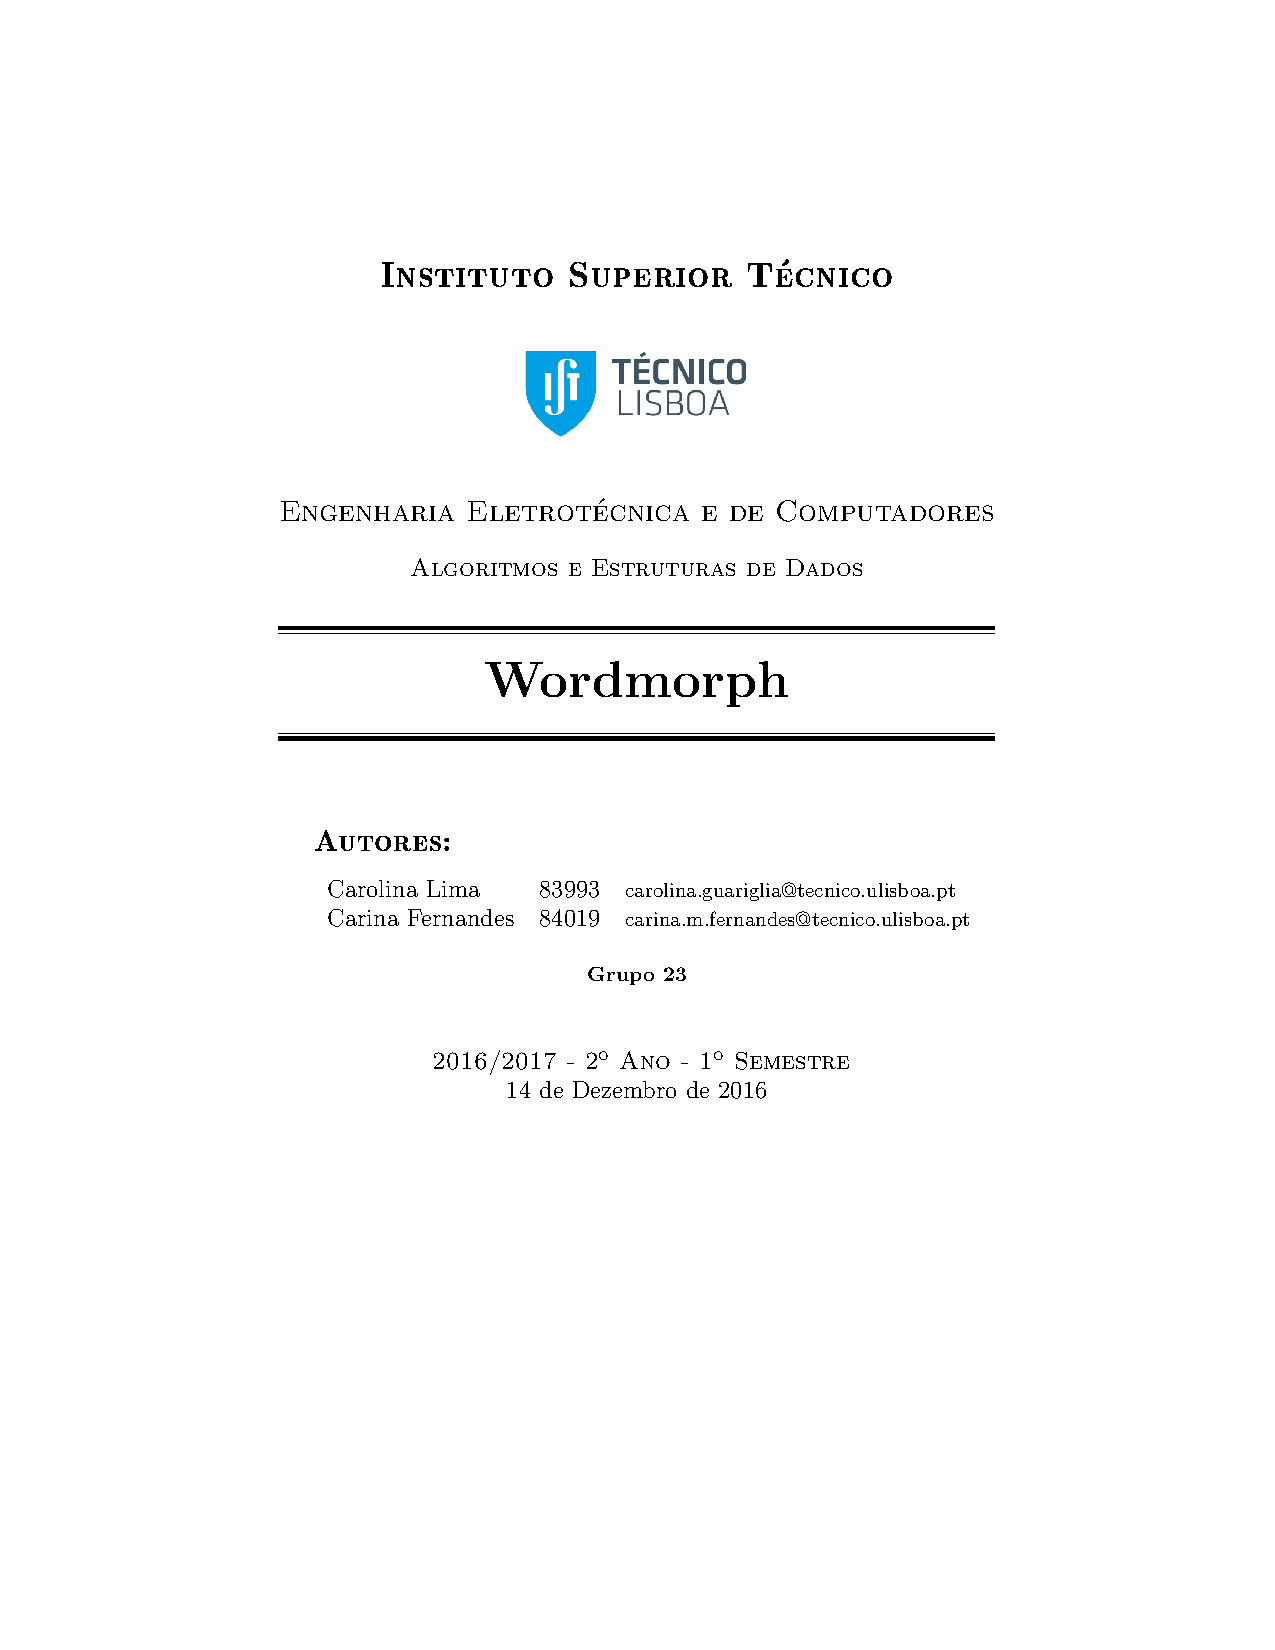
\includepdf[pages={1}]{capa/capa.pdf}

\pagestyle{fancy}
\tableofcontents
\newpage

\section{Descrição do problema}
    \par O problema enunciado consiste na procura de caminhos entre palavras. Estes caminhos são, na verdade, uma sequência de palavras de tamanho igual no qual cada palavra se obtêm mudando uma ou mais letras da palavra anterior, até chegar à palavra desejada. Para além disso, todas as palavras pertencentes ao caminho têm obrigatoriamente de pertencer a um dicionário. Dicionário é definido neste caso como uma lista de palavras, que não têm obrigatoriamente de ser todas do mesmo tamanho.
    \par Como é possível a existência de vários caminhos, distingue-se cada passo do caminho pelo número de caracteres que são mudados. No fim, os custos dos caminhos somam-se para chegar ao custo final. Por exemplo, um passo no qual se mude um caracter têm o custo de $1^1$, um passo em que se mudam dois caracteres têm um custo de $2^2$, e assim sucessivamente.
    \par O objectivo final deste projecto é, dado duas palavras e o número máximo de trocas que se podem efectuar em cada passo, retornar o caminho de menor custo entre essas duas palavras.
    
\section{Abordagem do problema}
    \par Para resolver o problema, decidiu-se dividi-lo nas seguintes partes: guardar as palavras do dicionário e procurar o caminho propriamente dito. Chegou-se então à conclusão de que seria necessário guardar as palavras do dicionário num local que fosse facilmente acessível, e que não seria necessário guardar todas as palavras, apenas as relevantes, tal como não é necessário fazer todos os grafos.
\subsection{Procura do caminho de menor custo}
    \par A escolha óbvia para resolver este problema foi recorrer ao algorítmo de Dijkstra, que procura o caminho mais curto entre dois vértices de um dado grafo desde que nenhuma das arestas do mesmo tenha peso negativo, o que é o caso deste problema. Para podermos utilizar então o algorítmo, chegou-se então à conclusão que é necessária a criação de um grafo representado por listas de adjacências (o algorítmo não é igual para matrizes de adjacência).
    
\section{Implementação do programa}
    \par Dividiu-se então o programa em três partes distintas: uma parte referente às estruturas de dados, uma parte que se relaciona diretamente com o problema a resolver, e por fim todas as restantes operações que não pertencem a nenhum dos anteriores grupos. No código, estas partes equivalem aos ficheiros datastructs.c, words.c e utils.c respectivamente.
    \par Para evitar alocações de memória desnecessárias, percorrem-se todas as linhas do ficheiro de dicionário duas vezes. Uma para contar o número de palavras que existem de cada tamanho de palavra, outra para copiar as palavras do ficheiro para a matriz que representa o dicionário, cujo tamanho é alocado baseando-se no número obtido anteriormente. Assumiu-se que nunca existiriam palavras de mais de cem letras.
    \par Como mencionado na secção anterior, rapidamente chegou-se à conclusão de que é desnecessário criar grafos que não vão ser utilizados. Por isso, também percorre-se uma vez pelo ficheiro de problemas sem os começar a resolver, para saber que tamanhos de palavras existem no ficheiro, e qual número máximo de caracteres que mudam entre duas palavras do caminho.
    \par Assim, decidiu-se estruturar o programa como esquematizado no fluxograma da figura \ref{fig:flux1}.
    
    \begin{figure}
        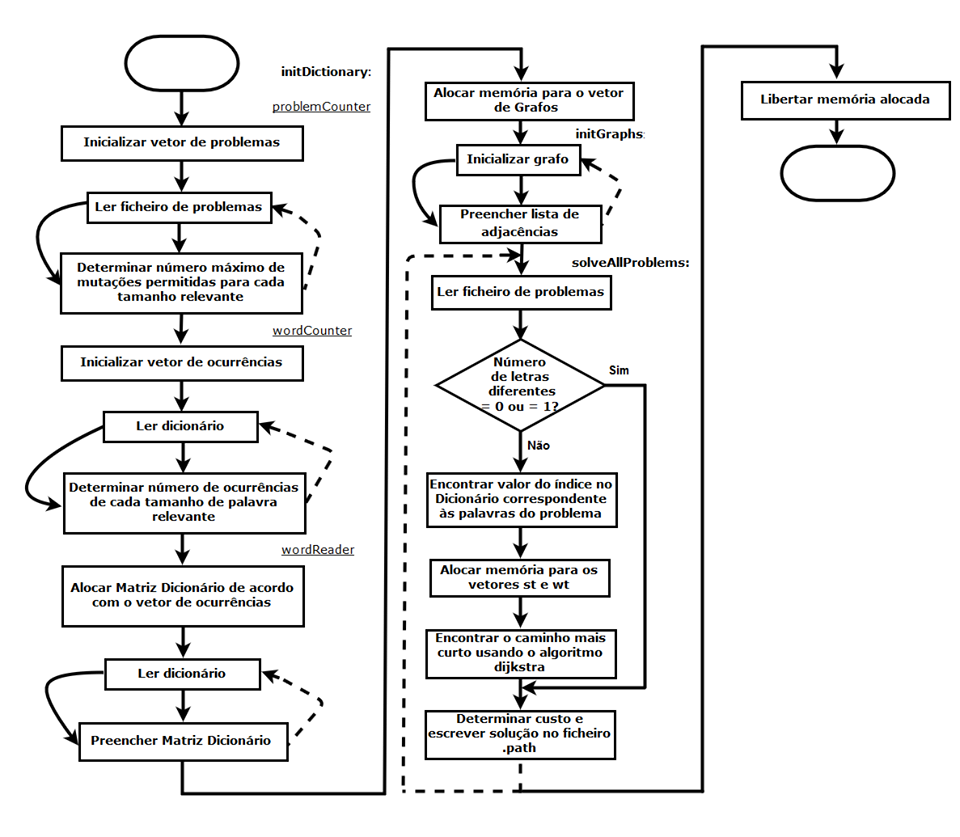
\includegraphics[width=\linewidth]{fluxograma1.png}
        \caption{Fluxograma da função problemSolver}
        \label{fig:flux1}
    \end{figure}
    
\subsection{Descrição das estruturas de dados}
    \par A estrutura de dados que foi considerada a mais adequada para guardar o dicionário foi uma matriz, ou seja um vector de vectores, para diminuir os custos de memória e de acesso.
    \par Como referido acima, foi claro que seria necessária a representação do grafo tendo como base uma lista de adjacências, então foi implementada uma lista genérica. Esta é definida usando $void *$ (definido em datastructs.h, e a partir daqui referido como Item), para os quais se pode passar qualquer ponteiro, assegurando a generalidade da implementação. O grafo em si é um grafo adirecional e acíclico, o que facilitou a implementação.
    \par As listas definidas foram então utilizadas na definição do grafo pois este é implementado usando uma lista de adjacências. Os grafos foram definidos de forma genérica, com um reparo - a implementação dos dados usados na lista estão visíveis ao cliente. Todos os novos elementos desta lista são inseridos na primeira posição (head).
    \par Como terá de existir um grafo para cada tamanho de palavras, decidiu-se usar um vetor para guardá-los no qual o índice corresponde ao tamanho das palavras representadas no grafo (i.e. all{\_}arrays[3] contêm o grafo das palavras de tamanho 3).
    \par Por fim, a descrição do algorítmo de Dijkstra requer um acervo, também este definida de forma genérica no código. Neste caso, o acervo foi implementado usando uma fila prioritária, que por sua vez foi implementada usando um vector. Este vector tem um tamanho fixo, definido na sua incialização, mas usou-se outra vaŕiavel (q$\rightarrow$first) para que exista um ``vector virtual''  dentro do vector maior. Outra das variáveis que foi útil foi um vector indexado por vértices que diz onde o vértice está na heap (q$\rightarrow$vert{\_}pos), que evita que se tenha de fazer procura linear cada vez que se quer encontrar um vértice na heap.
    
\subsection{Descrição dos algoritmos utilizados}
    \par O algorítmo utilizado para a criação do grafo é de complexidade $O(n^2)$, visto que não foi possível encontrar uma solução mais simples computacionalmente. Porém, não é necessário comparar todas as palavras a todas as palavras se se usar o algorítmo descrito pelo pseudo-código abaixo:
    
    \begin{center}
        \texttt{\begin{tabular}{l}para i pertencente ao dicionário: \\
        \quad para todo j < i: \\
        \quad\quad se i e j tiverem menos letras diferentes do que o custo máximo \\
        \quad\quad\quad ligar j a i \\
        \quad\quad\quad ligar i a j\\\end{tabular}}
    \end{center}
    
    \par Este código reduz a complexidade do algorítmo de criação do grafo para $O(\frac{n^2}{2})$, o que não é ideal mas é melhor do que a alternativa.
    
    \par Mas claramente, o algorítmo crucial ao programa foi o algoritmo de Dijkstra, usando a variação que encontra o caminho mais curto entre dois vértices e não a que encontra o caminho mais curto entre um vértice e todos os outros vértices do grafo, ou seja, parando quando o elemento que sai da heap é o vértice a que se quer chegar.
    
    \par Por fim, para a impressão da solução do problema para o ficheiro foram utilizados mais dois algorítmos: um para calcular o custo total e um para descobrir qual o caminho mais curto a partir do vector st, que é um argumento da função que implementa o algorítmo de Dijkstra.
    \par O cálculo do custo consiste de com o vector st, descobrir todos os passos da solução (a ordem dos passos é indiferente). Assim, soma-se então o custo de cada passo até que o valor do vector st seja -1, ou seja, que se tenha chegado ao vértice inicial. A impressão do custo teve de ser pensada de forma diferente, visto que a ordem interessa neste caso. Por isso, para garantir que os resultados estariam correctos, considerou-se que a forma mais simples seria implementar recorrendo a um algorítmo recursivo.
    \par Este algorítmo, sendo recursivo, necessita de uma condição de saída. Neste caso, a função retorna sem chamar-se a si mesma se argumento passado equivale ao índice do array que representa o vértice original. Caso esta condição não se verifique, a função chama-se a si mesma e imprime a palavra equivalente para o ficheiro de saída.
    
\section{Subsistemas funcionais}
    \par Como já referido, existem três subsistemas funcionais:
    \begin{description}[align=left]
       \item[datastructs.c] Implementa os três tipos de dados essenciais - listas ligadas, grafos e acervos. Inclui as funções requiridas por cada tipo de dados, como a inicialização, libertação de memória e funções de interface para que o cliente possa interagir com as estruturas.
       \item[utils.c] Funções variadas que não fariam sentido estar noutro ficheiro. Tem funções que lidam com a abertura de ficheiros, comparações, e a implementação do algorítmo de Dijkstra.
       \item[words.c] Encontra-se tudo que se relaciona diretamente com a resolução do problema, como por exemplo a determinação da maior permutação e a leitura das palavras dos ficheiros de dicionário e problemas.
    \end{description}
    
\subsection{datastructs.c}
    \begin{itemize}
    \end{itemize}
    
\subsection{utils.c}
    \begin{itemize}
    \item void * allocate(size{\_}t);
    \par Função que funciona como o malloc mas com verificação de erros.
    
    \item FILE * fcheck(char *, char *);
    \par Verifica se um ficheiro tem uma determinada extensão e abre-o de seguida.
    
    \item char* outputFileExtension(char * name{\_}input);
    \par Dado o nome de um ficheiro, retorna o nome do ficheiro com uma extensão diferente (a extensão está \textit{hard-coded}).
    
    \item int calculateDifferentLetters(char *word1, char *word2, int cost);
    \par Dadas duas palavras, calcula o número de letras diferentes entre elas. O parâmetro cost é uma otimização - se o custo já ultrapassar o custo máximo que se quer calcular já não vale a pena iterar pela palavra.
    
    \item int compInts(Item i1, Item i2);
    \par Dados dois inteiros, retorna 1 se o primeiro for maior do que o segundo, -1 se o segundo for maior do que o primeiro e 0 se forem iguais.
    
    \item int compWeight(Item item1, Item item2);
    \par De forma semelhante à função acima, dados dois g{\_}datas, retorna 1 se o peso do primeiro for maior do que o segundo, -1 se o peso do segundo for maior do que o primeiro e 0 se os pesos forem iguais.
    
    \item void lowerWeight(queue *q, int idx, Item new{\_}weight);
    \par Serve para baixar a prioridade de algo numa fila prioritária - neste caso, baixa o peso de um elemento da fila.
    
    \item void dijkstra(graph *g, int s, int end, int max{\_}step, int *st, int *wt);
    \par Implementa o algorítmo de Dijkstra, usando uma fila prioritária.
    
    \item void writefirstOutput(FILE * fp, char * word, int cost);
    \par Escreve a primeira linha da solução para o ficheiro, visto que é diferente das restantes.
    
    \item void writeOutput(FILE * fp, char * word);
    \par Escreve uma linha da solução para o ficheiro.
    
    \item void freeMatrix(char ***mat, int *size, int init{\_}size);
    \par Liberta uma matriz de caracteres. Note-se que assume-se que o tamanho da matriz pode ser variável, por isso é que se passa o vector size.
    
    \end{itemize}

\subsection{words.c}

    \begin{itemize}
    \item void problemCounter(FILE *prob, int *problem{\_}array);
    \par Itera pelo ficheiro de problemas, contando qual a iteração máxima para cada tamanho de palavra.
    
    \item void wordCounter(FILE *input, int *occurrences, int *problems);
    \par Itera pelo ficheiro de dicionário, contando quantas palavras de cada tamanho existem. Só conta tamanhos de palavras relevantes para a resolução do problema.
    
    \item void wordReader(FILE *input, char **output[MAX{\_}STRING], int *size{\_}array);
    \par Sabendo quantas palavras existem de cada tamanho, guarda as palavras relevantes para a resolução numa matriz de caracteres.
    
    \item void initDictionary(FILE *prob, FILE *dic, char **dictionary[MAX{\_}STRING], int *to{\_}solve, int *word{\_}count);
    \par Chama as três funções descritas acima, para facilitar a criação da matriz de palavras.
    
    \item void initGraphs(graph **all{\_}graphs, int *max{\_}change, int *size{\_}array, char ***dict);
    \par Inicializa os grafos necessários para a resolução do problema, tendo em conta a permutação máxima entre palavras.
    
    \item void printPath(FILE *output, int w{\_}size, int *st, int origin{\_}v, int final{\_}v, char **dic[MAX\-{\_}STRING], int cur);
    \par Imprime o caminho entre duas palavras, usando um algorítmo recursivo. Não imprime nem a primeira nem a última palavra.
    
    \item int calculateTotalCost(int *st, int final{\_}v, char **dic);
    \par Calcula o custo total do caminho, dado o vector st e o vértice final.
    
    \item void solveAllProblems(FILE *input, FILE *output, graph **all{\_}graphs, char **dictionary[MAX\-{\_}STRING], int *size{\_}array);
    \par  Itera pelos problemas do ficheiro, lida com eles da forma apropriada (chamando ou não o algorítmo de Dijkstra) e chama as funções que escrevem os resultados para o ficheiro.
    
    \item void problemSolver(FILE *dic, FILE *prob, FILE *path);
    \par A função principal do problema - chama as funções que criam os grafos, o dicionário, que resolvem os problemas e que libertam a memória.
    
    \item void freeAllGraphs(graph **all{\_}graphs);
    \par Resolvidos todos os problemas, liberta os grafos um a um seguidos do vector que os guardava.
    
    \end{itemize}

\section{Complexidade do programa}
    \par Examinando o programa, chega-se à conclusão de que existem duas grandes partes que contribuem para a complexidade. Em ambos os casos, $v$ representa o número total de palavras com o mesmo tamanho e $e$ representa o número de ligações que existem entre palavras.
    \begin{description}[align=left]
        \item[Criação de grafo] Para inserir todas as palavras no grafo, é necessário comparar todas as palavras duas a duas. No código, como para cada palavra do dicionário só é necessário comparar as palavras anteriores a esta, o que acontece é $1 + 2 + 3 + ... + v = \frac{v^2}{2} + \frac{v}{2}$, que é majorado por $v^2$ concluindo-se então que a complexidade será $O(v^2)$.
        \par Em termos de memória, a complexidade será de $O(e^2)$, visto que numa lista de adjacências de um grafo não direccionado uma ligação é reperesentada por dois nós.
        \item[Algorítmo de Dijkstra] No caso do problema a resolver, observa-se que o grafo que representa as ligações é um grafo esparso (menos do que $|v^2|$ ligações). Assim, esta implementação do algorítmo de Dijkstra, usando uma lista de adjacências e um acervo, corre em $\Uptheta((|e| + |v|)log(|v|))$, como há uma estrutura de dados auxiliar que indica aonde está cada vértice na heap, fazendo com que a procura seja $O(1)$.
    \end{description}

\section{Análise do programa}
    \par Na supefície, o problema é simples - no entanto é necessária alguma cautela para alguns casos limite e para alguns descuidos que podem aumentar e muito o tempo de execução do problema. Um destes descuidos foi a procura de um determinado vértice dentro da \textit{heap} - a abordagem \textit{naïve} utilizada inicialmente tinha complexidade $O(n)$, o que considando as vezes que era necessário descobrir o vértice, ``estragava'' a rapidez do algorítmo de Dijkstra.
    \par Outro problema, que foi mais trivial de resolver, foi o facto de que não foram antecipados certos tipos de problemas, nomeadamente que a palavra de partida fosse igual à palavra de chegada e que a diferença entre as palavras fosse apenas de uma letra.

\section{Exemplo}
    \par De seguida será ilustrado o funcionamento do programa de forma a demonstrar o racíocinio implementado, acima descrito. 
    \par É de notar que se pressupõe que o ficheiro .dic se trata de um ficheiro com palavras não acentuadas, sem hífen, separadas por espaços ou \textit{newlines} e que inclui todas as palavras que se encontram no ficheiro de problemas. Sendo o ficheiro de dicionário deste tipo, com nome dexemplo.dic:
        \begin{center}
        \texttt{\begin{tabular}{l}gotas bisturi agente corpo \\
        pausa trampolim parte zebra casta \\
        cobertor liberdade casto gorro  \\
        ...
        \end{tabular}}
        \end{center}
           
    \par Em relação ao ficheiro .pal é então presumido, por sua vez, que este contem para cada problema duas palavras do mesmo tamanho e um inteiro, sendo este o custo associado ao caminho. Sendo este pexemplo.pal:
        \begin{center}
        \texttt{\begin{tabular}{l}aguenta aguento 3 \\
        gotas casta 3 \\
        cobertor cobertor 4 \\
        zebra pausa 2
        \end{tabular}}
        \end{center}
        
    \par O programa desenvolvido irá antes de mais confirmar as extensões dos ficheiros introduzidos na linha de comandos. Visto que ambos possuem a extensão correta será criado o nome do ficheiro de saída com o mesmo do .pal mas com a extensão .path, ou seja pexemplo.path.
	\par De seguida será lido o ficheiro pexemplo.pal e criado um vetor, problem{\_}array, inicializado a zero com tamanho MAX{\_}STRING = 100, com o custo máximo de mutação para cada tamanho de palavra representado no ficheiro de problemas relevante à resolução. 
    Isto é, na posição 5 terá o valor 3 visto ser a mutação máxima permitida entre palavras de tamanho 5 e tanto na posição 6 como na 8, manterão o valor 0 visto que os únicos problemas envolvendo palavras de tamanho 6  e de tamanho 8 podem ser resolvidos diretamente sem a necessidade de grafos. Na função seguinte será preenchido o vetor de número de ocurrências de tamanhos de palavras no ficheiro .dic, estando este inicializado a zero. 
	\par Visto que o único tamanho com um valor na posição respectiva do problem{\_}array maior que zero é o 5 serão contadas o número de palavras de tamanho 5 no ficheiro, ficando então na posição 5 deste vetor o valor 7.
	\par Seguidamente será então criada a matriz que representa o dicionário, que terá, na posição 5:
	
		\begin{center}
        \texttt{gotas \\ corpo \\ pausa \\ parte \\ 
        zebra \\ casto \\ gorro \\
        }
        \end{center}
	
	\par Após alocada memória para um vetor de grafos, que apenas irá conter um grafo com as palavras de tamanho 5, será preenchida a sua lista de adjacência tendo cada palavra na sua lista apenas palavras que dela diferem 3 ou menos caracteres.
	
        \begin{center}
        \texttt{\begin{tabular}{l}Adj[0] para gotas : gorro \\
        Adj[1] para corpo : gorro -> casto \\
        Adj[2] para pausa : parte \\
        Adj[3] para parte : casto -> pausa \\
        Adj[4] para zebra : NULL \\
        Adj[5] para casto : parte -> corpo \\
        Adj[6] para gorro : corpo -> gotas
        \end{tabular}
        }
        \end{center}
	
	\par Agora que já foi o grafo necessário à resolução do problema será lido o ficheiro .pal e resolvidos os problemas um a um. Para o primeiro as palavras do problema apenas apresentam uma diferença de um caracter, sendo então a sua solução imediatamente escrita no ficheiro .path como:
	
		\begin{center}
        \texttt{\begin{tabular}{l}aguenta 1\\
				aguento\\
        \end{tabular}}
        \end{center}
	
	\par Para o segundo problema o mesmo já não se verifica sendo portanto necessaŕio recorrer ao algorítmo de Dijkstra. Antes de mais, serão comparadas as palavras do problema com as do mesmo tamanho inseridas no dicionário, de modo a determinar o valor do vértice inicial e final correspondente ao índice destas palavras no vetor de palavras do mesmo tamanho contido na matriz que representa o dicionário.
	\par Neste caso o vértice inicial terá o valor 0 e o final o valor 5. 
	
	\par Já no algoritmo será inicalizada o acervo, cujos vetores terão ambos um tamanho inicial de 7, sendo o peso de cada vértice definido como MAX{\_}WT. Serão ainda inicializados os vetores st e wt, também de tamanho 7, com o valor -1 e MAX{\_}WT, respetivamente. O peso do vértice inicial 0, tanto no acervo como no vetor wt, passará para 0 e será de seguida realizado o fixUp do acervo para o restaurar.
	\par Na tabela \ref{ac} apresenta-se uma ilustração da evolução do acervo ao longo do algoritmo.	
	
    \begin{table}
        \begin{center}
        \begin{tabular}{llllllllllllll}
            \multicolumn{7}{l}{\textbf{Acervo Inicializado:}}                                                                          & 0          & 1          & 2          & 3          & 4          & 5          & 6          \\
        \multicolumn{7}{l}{\textbf{Após alterada prioridade:}}                                                                     & \textbf{0} & \textbf{1} & \textbf{2} & \textbf{3} & \textbf{4} & \textbf{5} & \textbf{6} \\
        \multicolumn{7}{l}{Removido o de menor peso:}                                                                              & 1          & 3          & 2          & 6          & 4          & 5          &            \\
        \multicolumn{7}{l}{\begin{tabular}[c]{@{}l@{}}st[6] = 0 ; wt[6] = 9\\ Depois de alterado e realizado FixUp:\end{tabular}}  & 6          & 1          & 2          & 3          & 4          & 5          &            \\
        \multicolumn{7}{l}{Removido o de menor peso:}                                                                              & 1          & 3          & 2          & 5          & 4          &            &            \\
        \multicolumn{7}{l}{\begin{tabular}[c]{@{}l@{}}st[1] = 6 ; wt[1] = 13\\ Depois de alterado e realizado FixUp:\end{tabular}} & 1          & 3          & 2          & 5          & 4          &            &            \\
        \multicolumn{7}{l}{Removido o de menor peso:}                                                                              & 3          & 5          & 2          & 4          &            &            &            \\
        \multicolumn{7}{l}{st[5] = 1 ; wt[5] = 22}                                                                                 &            &            &            &            &            &            &            \\
        \multicolumn{7}{l}{}                                                                                                       &            &            &            &            &            &            &
        \end{tabular}
        \caption{Evolução do acervo para o problema 2}
        \label{ac}
        \end{center}
    \end{table}
	
	\par É de notar que após a remoção do vértice de menor peso do acervo, serão verificados os vértices seus adjacentes para a otimização do caminho. Isto é, depois de retirado o vértice 0 será analisado o vértice 6 que apresenta um melhor caminho passando este a ser o de menor peso no acervo. Analogamente será considerado o vértice 1 e por fim o vértice 5 que corresponde ao vértice final.
	\par Quando o vértice retirado do acervo corresponder ao vértice final é possível então terminar este processo, estando o caminho representado no vetor st. 
	
	\par O vetor st obtido está representado na tabela \ref{vct}.
    
    \begin{table}[]
	\centering
	\begin{tabular}{|l|c|c|c|c|c|c|c|}
    \hline
	Índice: & 0  & 1 & 2  & 3  & 4  & 5 & 6 \\ \hline
	st {[} Índice {]}: & -1 & 6 & -1 & -1 & -1 & 1 & 0 \\ \hline
	\end{tabular}
    \caption{Vetor st solução do problema 2}
	\label{st2}
	\end{table}
    
    \par Obtido este vetor será impresso o caminho no ficheiro .path, sendo esta escrita realizada rescursivamente. 
	
	\begin{center}
        \texttt{\begin{tabular}{l}gotas 22\\
			gorro\\
			corpo\\
			casto\\
        \end{tabular}}
        \end{center}
	
	
	\par Para o terceiro problema a situação é trivial e análoga à do primeiro problema, visto que as duas palavras são iguais, sendo portanto resolvida diretamente e impressa no ficheiro .path como:
	
	\begin{center}
        \texttt{\begin{tabular}{l}cobertor 0\\
		cobertor
        \end{tabular}}
    \end{center}
        
    \par O quarto problema é, por sua vez, análogo ao segundo problema, estando a evolução do acervo representada na Tabela \ref{acv4}.
    
    \begin{table}[]
	\centering
	\begin{tabular}{llllllllllllll}
	\multicolumn{7}{l}{\textbf{Acervo Inicializado:}}      & 0          & 1          & 2          & 3          & 4          & 5          & 6          \\
	\multicolumn{7}{l}{\textbf{Após alterada prioridade:}} & \textbf{4} & \textbf{0} & \textbf{2} & \textbf{3} & \textbf{1} & \textbf{5} & \textbf{6} \\
	\multicolumn{7}{l}{Removido o de menor peso:}          & 0          & 3          & 2          & 6          & 1          & 5          &            \\
	\multicolumn{7}{l}{Removido o de menor peso:}          & 3          & 6          & 2          & 5          & 1          &            &            \\
	\multicolumn{7}{l}{Removido o de menor peso:}          & 6          & 5          & 2          & 1          &            &            &            \\
	\multicolumn{7}{l}{Removido o de menor peso:}          & 5          & 1          & 2          &            &            &            &            \\
	\multicolumn{7}{l}{Removido o de menor peso:}          & 1          & 2          &            &            &            &            &            \\
	\multicolumn{7}{l}{Removido o de menor peso:}          & 2          &            &            &            &            &            &           
	\end{tabular}
	\caption{Evolução do acervo para o problema 4}
	\label {acv4}
	\end{table}
		
	\par Neste caso não foi encontrado um caminho que satisfizesse o custo máximo permitido entre mutações, isto é, no máximo 2 caracteres de uma vez.	
    
    \begin{table}[]
	\begin{center}
	\begin{tabular}{|l|c|c|c|c|c|c|c|}
    \hline
	Índice: & 0  & 1 & 2  & 3  & 4  & 5 & 6 \\ \hline
	st {[} Índice {]}: & -1 & -1 & -1 & -1 & -1 & -1 & -1 \\
    \hline
	\end{tabular}
    \caption{Vetor st solução do problema 4}
    \label{vct}
    \end{center}
	\end{table} 
	
	\par Obtido este vetor será indicado no ficheiro .path a inexistência de caminho da seguinte forma:
    
    \begin{center}
        \texttt{\begin{tabular}{l}zebra -1 \\
        pausa
        \end{tabular}}
    \end{center}

\section{Bibliografia}


\end{document}
